%%%%%%%%%%%%%%%%%%%%%%%%%%%%%%%%%%%%%%%%%
% Beamer Presentation
% LaTeX Template
% Version 1.0 (10/11/12)
%
% This template has been downloaded from:
% http://www.LaTeXTemplates.com
%
% License:
% CC BY-NC-SA 3.0 (http://creativecommons.org/licenses/by-nc-sa/3.0/)
%
%%%%%%%%%%%%%%%%%%%%%%%%%%%%%%%%%%%%%%%%%

%----------------------------------------------------------------------------------------
%	PACKAGES AND THEMES
%----------------------------------------------------------------------------------------

\documentclass{beamer}

\mode<presentation> {

% The Beamer class comes with a number of default slide themes
% which change the colors and layouts of slides. Below this is a list
% of all the themes, uncomment each in turn to see what they look like.

%\usetheme{default}
%\usetheme{AnnArbor}
%\usetheme{Antibes}
%\usetheme{Bergen}
%\usetheme{Berkeley}
%\usetheme{Berlin}
%\usetheme{Boadilla}
%\usetheme{CambridgeUS}
%\usetheme{Copenhagen}
%\usetheme{Darmstadt}
%\usetheme{Dresden}
%\usetheme{Frankfurt}
%\usetheme{Goettingen}
%\usetheme{Hannover}
%\usetheme{Ilmenau}
%\usetheme{JuanLesPins}
%\usetheme{Luebeck}
\usetheme{Madrid}
%\usetheme{Malmoe}
%\usetheme{Marburg}
%\usetheme{Montpellier}
%\usetheme{PaloAlto}
%\usetheme{Pittsburgh}
%\usetheme{Rochester}
%\usetheme{Singapore}
%\usetheme{Szeged}
%\usetheme{Warsaw}

% As well as themes, the Beamer class has a number of color themes
% for any slide theme. Uncomment each of these in turn to see how it
% changes the colors of your current slide theme.

%\usecolortheme{albatross}
%\usecolortheme{beaver}
%\usecolortheme{beetle}
%\usecolortheme{crane}
%\usecolortheme{dolphin}
%\usecolortheme{dove}
%\usecolortheme{fly}
%\usecolortheme{lily}
%\usecolortheme{orchid}
%\usecolortheme{rose}
%\usecolortheme{seagull}
%\usecolortheme{seahorse}
%\usecolortheme{whale}
%\usecolortheme{wolverine}

%\setbeamertemplate{footline} % To remove the footer line in all slides uncomment this line
%\setbeamertemplate{footline}[page number] % To replace the footer line in all slides with a simple slide count uncomment this line

%\setbeamertemplate{navigation symbols}{} % To remove the navigation symbols from the bottom of all slides uncomment this line
}

\usepackage{graphicx} % Allows including images
\usepackage{booktabs} % Allows the use of \toprule, \midrule and \bottomrule in tables

%----------------------------------------------------------------------------------------
%	TITLE PAGE
%----------------------------------------------------------------------------------------
\title[Statistical Learning]{Banded precision matrix tests} % The short title appears at the bottom of every slide, the full title is only on the title page

\author{Jiaming Shen} % Your name
\institute[UoM] % Your institution as it will appear on the bottom of every slide, may be shorthand to save space
{
University of Manchester \\ % Your institution for the title page
\medskip
\textit{jiaming.shen@postgrad.man.ac.uk} % Your email address
}
\date{\today} % Date, can be changed to a custom date

\begin{document}

\begin{frame}
\titlepage % Print the title page as the first slide
\end{frame}

\begin{frame}
\frametitle{Overview} % Table of contents slide, comment this block out to remove it
\tableofcontents % Throughout your presentation, if you choose to use \section{} and \subsection{} commands, these will automatically be printed on this slide as an overview of your presentation
\end{frame}

%----------------------------------------------------------------------------------------
%	PRESENTATION SLIDES
%----------------------------------------------------------------------------------------

%------------------------------------------------
\section{Introduction} % Sections can be created in order to organize your presentation into discrete blocks, all sections and subsections are automatically printed in the table of contents as an overview of the talk
%------------------------------------------------

%\subsection{Subsection Example} % A subsection can be created just before a set of slides with a common theme to further break down your presentation into chunks

\begin{frame}
\frametitle{Introduction}
Three approaches for test the bandwidth of the precision matrix is presented in this slides, which are An, Guo, \& Liu, (2014) work,Cheng, Zhang, \& Zhang (2017) and  Lee \& Lin (2018).
The main differences between this two is 
There are two main differences in constructing the test statistic.

\begin{enumerate}
\item An et al. (2014) use the modified cholesky decomposition
	while Cheng et al. (2017) didn't.
	
\item Cheng et al. (2017) sum up non-banded entry of the residual covariance matrix, while An et al. (2014) only sum up k-sub-diagonal entry.
\end{enumerate}

One main reason for such distinct is the Hypothesis are slightly different.

The hypothesis for Cheng et al. (2017) is ``Whether bandwidth is
\(\gamma\) or not''. The hypothesis for An et al. (2014) is
``\(K\leqslant k-1\)'' or ``\(K\leqslant k\)''.


\end{frame}

%------------------------------------------------

\begin{frame}
Another approach by Lee \& Lin (2018) is a similar method by An et al.
(2014), however he used Bayesian methods rather than the frequency
methods. Under the Bayesian set, the hypothesis is construct by bayes
factor rather than a statistics follow a certain distribution.

Lee \& Lee (2017) also showed a method using modified Cholesky
decomposition to estimate precision matrix. k-banded Cholesky prior

Lee \& Lin (2018) mainly concerned at the consistency of bandwidth
selection and Bayes factor. (However, I am not too care about this, I
mainly care about the methodology using to estimate the bandiwidth K and
the precision matrices.)

\end{frame}

\begin{frame}

Numbers of method will be benefit from the covariance structure modelling.
A example is the mean-covariance model
in longitudinal data by Pan \& Pan (2017) and (Pourahmadi, 2000)
analysis which involve the polynomial of time and lag-time to modelling
the covariance matrices. Another example is Lee \& Lin (2018) which use
the Gaussian DAG Models which has band-structured covariance/precision
matrices.
An et al. (2014) directly modelling the precision matrix in the multivariable Normal distribution without any specification application of the model.
Cheng et al. (2017)  consider the Undirected Graph which may refer as Markov random field.

\end{frame}

\begin{frame}
\

Not only for the LDA data, estimation of the covariance matrices is also
important for principle component analysis (PCA), linear/quadratic
distriminant analysis and multivariate analysis of variance (MANOVA)


n\textgreater{}\textgreater{}p case, sample covariance fails to converge
to the true covariance matrix (Johnstone, manuscript, \& 2004, n.d.).

\hypertarget{appendix-detail-notes-about-each-three-papers}{%
\subsection{Appendix : Detail notes about each three
papers}\label{appendix-detail-notes-about-each-three-papers}}
\end{frame}

\begin{frame}

Another from Lee \& Lin (2018) should be considered is Banerjee \&
Ghosal (2015) . This paper is mainly concern about the graphical model
structure, a sparse precision matrix of a Gaussian graphical model. The
edge presents or absences in a graphical model describing conditional
independence. A popular Non-Bayes method is graphical lasso. This paper
use bayesian method instead, use posterior distribution to learn the
covariance structure.G-Wishart prior is mentioned here.
\end{frame}


\begin{frame}
A very common question is rised here, why choosing banded structure, how to permutate the variable order to make the covariance matrix is banded? How to link the sparsity and the order to make a good explanation of a covariance matrix.

Or in other words, how to explore the structure may be the main concern before the hypothesis test.

Another question, if the stucture is sparse, are there any possibility to do some permutation to the matrix, change the order of variables can transfer the matrix to "banded like" or blocked diagonal matrices.
\end{frame}

\section{Bayesian Banded test}
\begin{frame}{The model specification:}
\subsubsection{The model specification:}
Gaussian DAG model by (Lee \& Lin, 2018) . 

DAG: Directed acyclic graph.

Direct graph: \(\mathcal { D } = ( V , E )\) ,V is vertices
\(V = \{ 1 , \ldots , p \}\) , E is directed edges. For any
\(i,j\in V\), \((i,j)\in E\) as a directed edge \(i\rightarrow j\).
There is no cycle in a DAG model. Assume parent ordering is known, where
\(i<j\) holds for any parent i of j in a DAG \(\mathcal D\). Gaussian
DAG model over \(\mathcal D\) :
\(Y = \left( Y _ { 1 } , \ldots , Y _ { p } \right) ^ { T } \sim N _ { p } \left( 0 , \Omega _ { n } ^ { - 1 } \right)\)
satisfies: \[
Y _ { i } \perp \left\{ Y _ { j } \right\} _ { j < i , j \in p a _ { i } ( \mathcal { D } ) }|  \left\{ Y _ { j } \right\} _ { j \in p a _ { i } ( \mathcal { D } ) }
\]

Consider,


\begin{align}
X _ { 1 },\ldots , X _ { n } | \Omega_{ n } \overset{i.i.d}{\sim} N _ { p } \left( 0 , \Omega _ { n } ^ { - 1 } \right)
\end{align}

\end{frame}

\begin{frame}
Cholesky Decomposition (Slight different from
Pourhmadi)

Do the Cholesky decomposition as following form : \[
\Omega _ { n } = \left( I _ { p } - A _ { n } \right) ^ { T } D _ { n } ^ { - 1 } \left( I _ { p } - A _ { n } \right)
\] with \(D_n=diag(d_j)\), \(a_{jj}=0\). Called \(A_n\) \emph{Cholesky
factor} is unique and lower triangular matrix. Result: \(a_{jl}\neq0\)
iff \(l\in pa_j(\mathcal D)\). Description: \(a_{jl}\) not 0 iff l is
parent of j, the edge \(l\rightarrow j\) exists. 
\end{frame}

\begin{frame}
Model: \[
\begin{array}
{ c } { X _ { i 1 } | d _ { 1 } \overset { i . i . d } { \sim } N \left( 0 , d _ { 1 } \right) } \\ 
{ X _ { i j } | a _ { j } ^ { ( k ) } , d _ { j } , k \overset { i n d } { \sim } N \left( \sum _ { l = ( j - k ) _ { 1 } } ^ { j - 1 } X _ { i l } a _ { j l } , d _ { j } \right) , \quad j = 2 , \ldots , p} 
\end{array}
\] That is, showed in above figure 
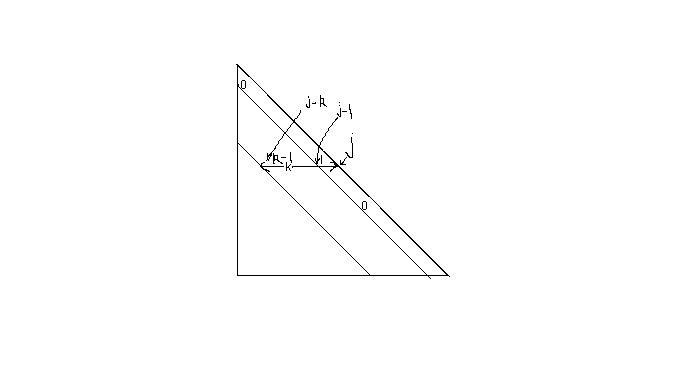
\includegraphics[width=5in]{bandedMatrix.png} 
\end{frame}




\begin{frame}
A very useful result: For Cholesky decomposition upon, the bandwidth of
\(A_n\) is k iff bandwidth of \(\Omega_n\) is \(k\).

Prior Distribution I'm not that concerned yet, however, should notice
that it is the conjugate prior. So the posterior distribution can be
calculated in a closed form up to some normalizing constant.

Assumption is important for the proof of estimation consistency,
however, I regards this is ``not neccessary'' for the idea of method, so
omit in this review. But I think the explaination in Section 2.4 is good
and worth reading if involve the proof of consistency and other
property.
\end{frame}


\begin{frame}

\subsubsection{Main result:}

\begin{enumerate}
\item
  Bandwidth selection consistency
\item
  Consistency of One-Sample Bandwidth Test Here construct a Bayesian
  bandwidth test for the testing problem: \[
  H_0:k\leqslant k^* \ \textit{vs }\ H_1:k>k^* 
  \] This is a composite hypothesis. The hypothesis test is based on the
  Bayes factor \(B_{10}(X_n)\) defined by the \textbf{ratio of marginal
  likelihoods} , \[
  B_{10}(X_{n})=\frac{p(X_n|H_1)}{p(X_n|H_0)}
  \] Denote the prior under the hypothesis \(H_i\) as
  \(\pi_i(A_n,D_n,k)\) for \(i=0,1.\) Using prior \(\pi_0(k)\) and
  \(\pi_1(k)\) such that \[
  \begin{array} { l l } { \pi _ { 0 } ( k ) = C _ { 0 } ^ { - 1 } \pi ( k ) , \quad k = 0,1 , \ldots , k ^ { * } } \\ { \pi _ { 1 } ( k ) = C _ { 1 } ^ { - 1 } \pi ( k ) , \quad k = k ^ { \star } + 1 , \ldots , R _ { n } } \end{array}
  \] with \(C _ { 0 } = \sum _ { k = 0 } ^ { k ^ { * } } \pi ( k )\),
  \(C _ { 1 } = \sum _ { k = k ^ { * } + 1 } ^ { R _ { n } } \pi ( k )\).
\end{enumerate}

\end{frame}

\begin{frame}
Then the Bayes factor (the statistic we construct for Hypothesis), is
  in analytic form, \[
  \begin{aligned} B _ { 10 } \left( \mathbf { X } _ { n } \right) & = \frac { \sum _ { k > k ^ { * } } \int p \left( \mathbf { X } _ { n } | \Omega _ { n } , k \right) \pi \left( \Omega _ { n } | k \right) \pi _ { 1 } ( k ) d \Omega _ { n } } { \sum _ { k \leq k ^ { * } } \int p \left( \mathbf { X } _ { n } | \Omega _ { n } , k \right) \pi \left( \Omega _ { n } | k \right) \pi _ { 0 } ( k ) d \Omega _ { n } } \\ & = \frac { \pi \left( k > k ^ { * } | \mathbf { X } _ { n } \right) } { \pi \left( k \leq k ^ { * } | \mathbf { X } _ { n } \right) } \times \frac { C _ { 0 } } { C _ { 1 } } \end{aligned}
  \] Consistency result: Under \(H_0:k\leq k^*\) \[
  B _ { 10 } \left( \mathbf { X } _ { n } \right) = O _ { p } \left( T _ { n , H _ { 0 } , k _ { 0 } , k ^ { * } } \right)
  \] Under \(H_1\) \[
  B _ { 10 } \left( \mathbf { X } _ { n } \right) ^ { - 1 } = O _ { p } \left( T _ { n , H _ { 1 } , k _ { 0 } , k ^ { * } } \right)
  \]
\end{frame}

\begin{frame}

Then is the method comparison between (An et al., 2014; Cheng et al.,
2017) and it's method. The mainly concern also is the consistency.

\begin{quote}
It is curious about the problem that how the test work, which means
significance under such bayes factor, such ratio?
\end{quote}

Quote from the arthor.

\begin{quote}
If \(H_0\) is true, \(B_{10}(Y)\) decreases at rate
\(O_p(e^{-c_0(k_2-k_1)})\) for some constant \(c_2>0\). On the other
hand, if \(H_1\) is true, \(B_{10}(Y)^{-1}\) decreases exponentially
with \(n(k_2-k_1)\beta^2_{min}\).
\end{quote}
\end{frame}

\begin{frame}

So there should be some threshold for the ratio about ``decline the
null-hypothesis'' or the ``accept the alter-hypothesis'' like 1 or 0.95
something. Back to the form of the Bayes factor :
\(B_{10}(X_{n})=\frac{p(X_n|H_1)}{p(X_n|H_0)}\) ,if \(H_0\) is true,
then the denominator is larger than the numerator, bayes factor is
closer to 0. If \(H_1\) is true, then numerator \(p(X_n|H_1)\) should be
larger than the denominator. Then the inverse of the Bayes factor should
closer to 0.

As {[}Bayes factor{]} (\url{https://en.wikipedia.org/wiki/Bayes_factor})
give a slightly discussion about the explaination of the bayes factor.
It seems no trivial maps from frequency 5\% level significance with test
under Bayes factor.

Because as it says, (An et al., 2014; Cheng et al., 2017)'s result is
that the statistic they constructed is asymptotically under Normal
distribution, then it comes to the normal 95\%
hypothesis-test-framework. Need notice, the asymptotically achieve for
\(n \wedge p \rightarrow \infty\) rather than \(n \rightarrow \infty\).
\end{frame}

\begin{frame}

\begin{quote}
Q : How the bayes factor linked with the Cholesky decomposition?
\end{quote}

\begin{quote}
A: Insider the analytic form of Bayes factor: \(p(X_n|\Omega_n,k)\) and
\(\pi(\Omega_n|k)\)
\end{quote}
\end{frame}

\begin{frame}

\begin{enumerate}
\setcounter{enumi}{2}
\item
  Two-Sample Bandwidth Test
\end{enumerate}

Problem: \[
\begin{array} { c } { X _ { 1 } , \ldots , X _ { n _ { 1 } } | \Omega _ { 1 n _ { 1 } } \stackrel { i . i . d . } { \sim } N _ { p } \left( 0 , \Omega _ { 1 n _ { 1 } } ^ { - 1 } \right)} \\ { Y _ { 1 } , \ldots , Y _ { n _ { 2 } } | \Omega _ { 2 n _ { 2 } } \stackrel { i . i . d } { \sim } N _ { p } \left( 0 , \Omega _ { 2 n _ { 2 } } ^ { - 1 } \right) } \end{array}
\] Interesting question: Test of equality between two bandwidths
\(k_1\)and \(k_2\). Hypothesis: \[
H _ { 0 } : k _ { 1 } = k _ { 2 },H _ { 1 } : k _ { 1 } \neq k _ { 2 }
\] Bayes factor: \[
B _ { 10 } \left( \mathbf { X } _ { n _ { 1 } } , \mathbf { Y } _ { n _ { 2 } } \right) = \frac { p \left( \mathbf { X } _ { n _ { 1 } } , \mathbf { Y } _ { n _ { 2 } } | H _ { 1 } \right) } { p \left( \mathbf { X } _ { n _ { 1 } } , \mathbf { Y } _ { n _ { 2 } } | H _ { 0 } \right) }
\]

\end{frame}


\begin{frame}

\begin{quote}
How to investigate the posterior/probability under the \(H_1\)
\(p(X_{n1},Y_{n_2})\)?
\end{quote}

To answer this question, should deep in P14 the construction and the
specifying of the prior distribution inside \(a_{1,j}^{(k_0)}\) and
\(a_{1,j}^{(k_1)}\) for given \(k_0\) and \(k_1\).

Then the Bayes factor can be written as analytic form under the prior
given \[
B _ { 10 } \left( \mathbf { X } _ { n _ { 1 } } , \mathbf { Y } _ { n _ { 2 } } \right) = \frac { \sum _ { k _ { 1 } \neq k _ { 2 } } \pi \left( k _ { 1 } | \mathbf { X } _ { n _ { 1 } } \right) \pi \left( k _ { 2 } | \mathbf { Y } _ { n _ { 2 } } \right) } { \sum _ { k _ { 1 } = k _ { 2 } } \pi \left( k _ { 1 } | \mathbf { X } _ { n _ { 1 } } \right) \pi \left( k _ { 2 } | \mathbf { Y } _ { n _ { 2 } } \right) } \times R _ { n } ^ { - 1 }
\]

Use marginal posterior distribution to deal with the alternative
hypothesis \(k_1\neq k_2\). And arthor gives a theorem about the
consistency of such test.

\end{frame}

\begin{frame}

Here start review about (An et al., 2014) . Summary about introduction.
(Will insert to begining of the final ediction of review.)

``When the data are multivariate Gaussian, the precision matrix can be
used to infer the conditional dependence structure of random
variables.'' Link between Precision matrix and conditional dependency
structure (Problem: Only for Gaussian? )

``When the variables of interest have a natural order, it is often
assumed that two random variable are not partially correlated when the
distance between the is large enough.'' It is interesting to do such
assumption, or just intuitively idea. There are things are done by this
sentence, one is the ``prior'' of the importantce of variable has order
and is already known. Then, the ``most interesting'' with ``less
interesting'' variable are less correlated. However, this may not true
in some situation, and may cause misleading in prior assumption.
\end{frame}

\begin{frame}
\begin{quote}
That is, another problem rised here, how to decide the order of the
variables, for banded structure, the covariance/precision matrix may
differ for \(X_1,X_2,...X_n\) from \(X_{i_1},...,X_{i_n}\) because the
banded covariance structure showed the dependency from a variable to
others is only on its neighbor. How to choose a satisfied order of
indeces \(I\) ? How about the precision matrices? (Under Gaussian is
same? How about other distributions?)
\end{quote}
\end{frame}

\begin{frame}{model-specification-notations}
\hypertarget{model-specification-notations}{%
\subsubsection{Model specification \&
Notations}\label{model-specification-notations}}

\(X _ { i } ( i = 1 , \dots , n )\) observation collected from the ith
subject.
\(X _ { i } = \left( X _ { i 1 } , \ldots , X _ { i p } \right) ^ { \mathrm { T } } \in \mathbb { R } ^ { p } ( i = 1 , \dots , n )\)
p-dimensional vector which are \emph{independent} and \emph{normally
distributed} with mean 0 and covariance matrix \(\Sigma\).

\begin{quote}
Notice: the collected data \(X\) is assume as multivariate Normal, and
without a respond Y, so it is \emph{NOT} a regression problem.
\end{quote}

MCD(modified cholesky decomposition) of \(\Sigma\) is denoted by
\(\Sigma = L D L ^ { \mathrm { T } }\), correspond formula in precision
matrix is \(\Omega = T ^ { \top } D ^ { - 1 } T\). Estimating \(T\),
\(D\) is equivelant to estimate \(\Omega\) and \(\Sigma\). 
\end{frame}

\begin{frame}
Similarly we
have the autoregressive property in such notation as \[
X _ { i j } = \sum _ { q = 1 } ^ { j - 1 } \left( - t _ { j q } \right) X _ { i q } + \varepsilon _ { i j }
\] for banded structure with bandwidth=\(K_0\) , we have \[
X _ { i j } = \sum _ { q = \left( j - K _ { 0 } \right) _ { 1 } } ^ { j - 1 } \left( - t _ { j q } \right) X _ { i q } + \varepsilon _ { i j }
\]

\end{frame}

\begin{frame}

Hypothesis: \[
H_0: K\leqslant k-1 \text{   vesus } H_1:K\geqslant k
\] k is prespecified positive number smaller than \(n-4\). Define
\(\mathcal { X } = \left( X _ { 1 } , \dots , X _ { n } \right) ^ { \mathrm { T } }\)
By fitting the autoregression equation, the estimator for \(t^{(k)}_j\)
as
\(\hat { t } _ { j } ^ { ( k ) } = - \left( \mathcal { X } _ { j } ^ { ( k ) \tau } \mathcal { X } _ { j } ^ { ( k ) } \right) ^ { - 1 } \mathcal { X } _ { j } ^ { ( k ) \mathrm { T } } \mathcal { X } _ { j }\).
Estimation for \(d_j\) as
\(\hat d_j^{(k)}=\left\| \mathcal { X } _ { j } + \mathcal { X } _ { j } ^ { ( k ) } \hat { t } _ { j } ^ { ( k ) } \right\| ^ { 2 } / \left[ n - \left\{ j - ( j - k ) _ { 1 } \right\} \right]\).

\begin{quote}
Surprise: finally an example that directly get the estimation by the
mcd.
\end{quote}
\end{frame}

\begin{frame}
\begin{quote}

Idea: can we do the autoregression between variables to obtain the
sparse covariance structure? such as
\(X_j=\sum_{i=1,i\neq j}^n \beta_i X_i\), test the significant to 0 for
\(\beta\) or regularized method to obtain the dependence structure for
\(X_1,...,X_n\sim N(0,\Sigma)\). Then we change the order of the
variables we can obtain a banded structure. Under such model, the
bandwidth may change, so can we develope a more specific test for
\(k_i\) ?

\end{quote}
\end{frame}

\begin{frame}

\emph{When \(H_0\) is true, then \(t_{j,j-k}=0\) for every \(j>k\). Then
the corresponding estimators should be small.} Follow this idea, the
test statistic is constructed as \[
L=\sum_{j=k+1}^p \hat t_{j,j-k}^{(k)2}
\]

The distribution, or approximate distribution of the test statistic is
needed for an accurate testing procedure.

From the construction, the statistic consider the difference between
``\(k\)-banded'' with ``\((k-1)\)-banded'', that is, showed in the
figure below:
\end{frame}

\begin{frame}
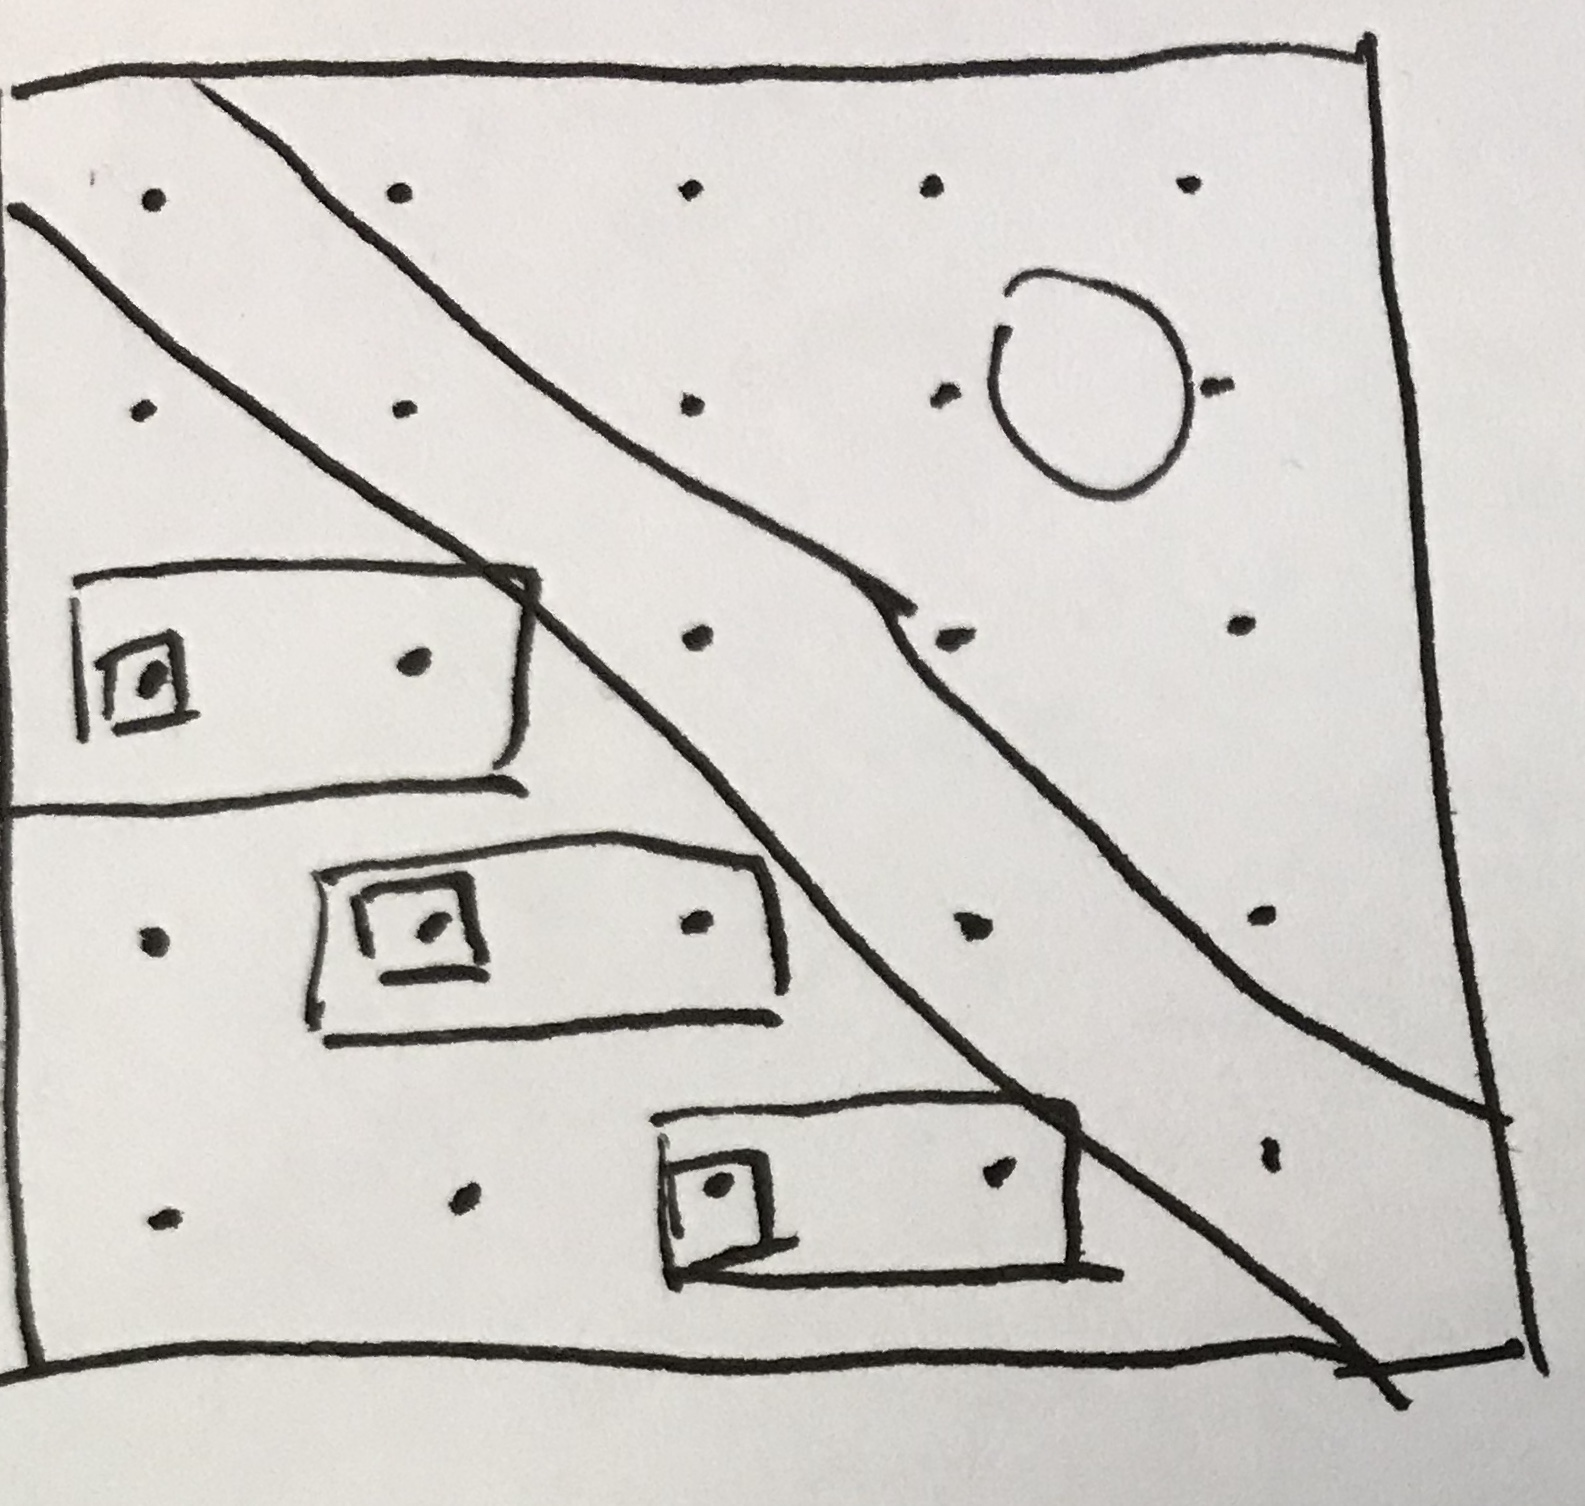
\includegraphics[width=2.5in]{Band_test_structure.jpg}

here is p=5,k=2 structure matrix.

The \(t^{(k)}_j\) is the rectangle box of vector, the statistics L is
the sum square of small square entry. It is the ``outer-wall'' of
k-banded with (k-1)-banded.
\end{frame}

\begin{frame}

Result by (Wu \& Pourahmadi, 2003): Conditonal on
\(\mathcal X_j^{(k)}\),
\(\hat t_{j,j-k}^{(k)}\sim N(t_{j,j-k},\Delta_j\hat d_j^{(k)})\) where
\(\Delta _ { j } = \left\{ \mathcal { X } _ { j - k } ^ { \mathrm { T } } \mathcal { X } _ { j - k } - \mathcal { X } _ { j - k } ^ { \mathrm { T } } \mathcal { X } _ { j } ^ { ( k - 1 ) } \left( \mathcal { X } _ { j } ^ { ( k - 1 ) \mathrm { T } } \mathcal { X } _ { j } ^ { ( k - 1 ) } \right) ^ { - 1 } \mathcal { X } _ { j } ^ { ( k - 1 ) \mathrm { T } } \mathcal { X } _ { j - k } \right\} ^ { - 1 }\).

We have \(\hat t_{j,j-k}^{(k)}\) is Normal, then the
\(\left( \Delta _ { j } \hat { d } _ { j } ^ { ( k ) } \right) ^ { - 1 / 2 } \left( \hat { t } _ { j , j - k } ^ { ( k ) } - t _ { j , j - k } \right)\sim t_{n-k}\).

Then
\(\left( \hat { t } _ { j , j - k } ^ { ( k ) } - t _ { j , j - k } \right) ^ { 2 } / \left( \Delta _ { j } \hat { d } _ { j } ^ { ( k ) } \right)\sim F_{1,n-k}\).

Take \(l_j\) defined as
\(\hat { t } _ { j , j - k } ^ { ( k ) 2 } / \left( \Delta _ { j } \hat { d } _ { j } ^ { ( k ) } \right)\)
, modified \(L\) as
\(L _ { c } = \sum _ { j = k + 1 } ^ { p } l _ { j }\)
\end{frame}

\begin{frame}

Even more, the variance may different for each j, from the
\(\hat t_j^{(k)}\) may different. Then need modified again by
standardize it. We have \(l_j\sim F_{1,n-k}\) with
\(E(l_j)=(n-k)/(n-k-2)\) and
\(var(l_j)=2(n-k)^2(n-k-1)/ \left\{ ( n - k - 2 ) ^ { 2 } ( n - k - 4 ) \right\}\)

\[
L _ { f } = ( p - k ) ^ { - 1 / 2 } \sum _ { j = k + 1 } ^ { p } \frac { l _ { j } - E \left( l _ { j } \right) } { \operatorname { var } \left( l _ { j } \right) ^ { 1 / 2 } }
\] Then the asymptotic null distribution of \(L_f\) as
\(n,p\rightarrow \infty\) is standard Normal.

After this, the arthor showed the power of the test.

Consider the hypothesis test below: \[
H _ { 0 k } : K \leqslant k - 1 \quad \text { versus } \quad H _ { 1 k } : K \geqslant k , \quad 1 \leqslant k \leqslant M
\] Then we can estimate bandwidth by
\(K_0=\{H_{0k} \text{ is false}\}\).

\end{frame}


\begin{frame}
Algorithm1:
\begin{enumerate}
\item
  Specify significance level \(\alpha\), upper bound of k: \(M\)
\item
  k=0, stop, output \(\hat K=k\),otherwise, compute the test-statistics
  \(L_f\) , denoted by \(L_f^{(k)}\). Let
  \(p_k=2\{1-\phi(|L_f^{(k)}|)\}\).
\item
  Test: if \(p_k>\alpha_k\), then do not reject \(H_{0k}\) , and update
  \(k=k-1\), back to Step 2. If \(p_k\leqslant \alpha_k\), reject
  \(H_{0k}\) and stop, report the bandwidth as \(\hat K=k\)
\end{enumerate}

Notice: This is a multiple comparison procedure, whould control each
\(\alpha_k\) in order to control overall significance level \(\alpha\).
Refer Efron (2010) for multiple comparison of hypothesis tests. Use
Bonferroni procedure sets \(\alpha_k=\alpha/M\) to control familywise
error so that it is no larger than \(\alpha\).

Bonferroni procedure may be too conservative when number of tests is
relative large. 

\end{frame}

\begin{frame}
Holm (1979) proposed following procedure:

Algorithm2:


\begin{enumerate}
\item
  Initialize \(\alpha\).
\item
  For k=1,\ldots{},M compute test statistics \(L_f^{(k)}\).
  \(p_k=2\{1-\phi(|L_f^{(k)}|)\}\)
\item
  Sort \(p_k\) as
  \(p _ { ( 1 ) } \leqslant \cdots \leqslant p _ { ( M ) }\) with
  correpond \(H_{0j_i},\cdots,H_{0j_M}\). Reject \(H_{0j_k}\) if
  \(p _ { ( j ) } \leqslant \alpha / ( M - j + 1 )\) for all
  \(j=1,...,k\).
\item
  No \(H_0\) is rejected: output \(\hat K=0\),implies diagonal matrix.
  Otherwise, \(\hat K=max\{k:H_{0k}\text{ is rejected}\}\).
\end{enumerate}
\end{frame}


\begin{frame}

Now start for review Cheng et al. (2017)

Data involve: genetic regulatory networks: gene expression data, medical
imaging, risk management and web search problems.

Data example: levels of \(p\) genes denotes as \((Y_1,...,Y_p)\) , a
concentration network can be described by an undirected graph in which
the p vertices represent the p genes and an edge connects gene i and
gene j iff the partial correlation \(\rho_{ij}\) between \(Y_i\) and
\(Y_j\).

Such model can describe by an undirected graph is which the pvertices
represent the p genes and an edge connects gene i and gene j if and only
if the partial correlation \(\rho_{ij}\) between \(Y_i\) and \(Y_j\) is
non-zero.
\begin{quote}
So in this description of undirected graph, the model is Markov random field ? 
\end{quote}
\end{frame}

\begin{frame}
Edge connected \(Y_i\) and \(Y_j\) iff partial correlation \(\rho_{ij}\)
is non-zero. If \(\left( Y _ { 1 } , \dots , Y _ { p } \right)\) are
jointly normally distributedm, estimating the structure of undirected
graph is equivalent to recovering the support of precision matrix
(\(\Omega=\Sigma^{-1}\))

\begin{quote}
Question: Just Gaussian graphical model for undirected model works? why
only undirect. (Lee \& Lin, 2018) is work on DAG, and (An et al., 2014)
is work on multi-variable Normal without any specification such as
graphical model.
\end{quote}

Normal property for this, see Lauritzen (1996) .
\end{frame}

\begin{frame}

Introduction part is interesting to collect wide range of papers.
(Bickel \& Levina, 2008) is very important, have to read it all.
(Rothman, Levina, \& Zhu, 2010) is also important, seems first use
Cholesky factor to model such covariance matrices. (But it seems too
late? But we should trust Biometrika). But seems I omit it for now.

\end{frame}

\begin{frame}{Notation and Model
specification}

\(\mathbf Y = (Y_1,...,Y_p)'\) : p-dimension vector sith mean \(\mu\)
and covariance matrix
\(\Sigma_y=(\sigma_{y,ij})_{p\times p}=\Omega^{-1}=(\omega_{ij})_{p\times p}\)

\(\mathcal B_{\gamma}\) is a class of banded matrices with bandwidth
\(\gamma\). A matrix \(\mathbf A=(a_{ij})\) is said to belong to
\(\mathcal B_{\gamma}\) if its elements (\(a_{ij}\)) are satisfies
\(a_{ij}=0\) if \(|i-j|>\gamma\). (The full-scale of bandwidth, then the
cholesky factor bandwidth should be \(\frac{\gamma}{2}\))

Hypothesis test problem: \[
H_{\gamma,0}:\Omega\in \mathcal B_\gamma \text{ vs. } H_{\gamma,1}:\Omega\notin \mathcal B_{\gamma}
\]
\end{frame}

\begin{frame}

Remark: Bickel \& Lindner (2012) showed: If \(\Omega\) belongs to
\(\mathcal B_\gamma\), there exists \(G_y\in B_{c\gamma}\) and
\(\Sigma_y\) can be approximated by \(G_y\) in the sense of
\(||\Sigma_y-G_y||\leq ( 1 / m ) ( ( M - m ) / ( M + m ) ) ^ { c }\)
(for every \(c\in N_0\)). \(||\cdot||\) is spectral norm. \(M\) and
\(m\) are largest and smallest eigenvalues of \(\Omega\). An efficient
method of testing the banded structure of \(\Sigma_y\) due to Qiu \&
Chen (2012) .


\end{frame}

\begin{frame}{Test Statistic:}



\(B _ { \gamma } ( \Omega ) = \left( \omega _ { i j } I \{ | i - j | \leq \gamma\} \right)\)
is a banded version of \(\Omega\) with bandwidth \(\gamma\). Then the
difference between \(\Omega\) and \(B_\gamma(\Omega)\) should be small
if null hypothesis is true.

The measurement of the difference between two matrices used in this
paper is matrix's Frobenius norm
\(\operatorname { tr } \left( \Omega - B _ { \gamma } ( \Omega ) \right) ^ { 2 }\).
Because it is easier to analysis.

Under the null hypothesis, then we have
\(\operatorname { tr } \left( \Omega - B _ { \gamma } ( \Omega ) \right) ^ { 2 } = \sum _ { | i - j | > \gamma } \omega _ { i j } ^ { 2 } = 0\)
\end{frame}

\begin{frame}

Let \[
Y_i=\alpha_i+Y'_{-i}\beta_i+\epsilon_i
\] \(\beta_i\) is a \(p-1\) vector
\(\left( \beta _ { 1 , i } , \ldots , \beta _ { i - 1 , i } , \beta _ { i + 1 , i } , \ldots , \beta _ { p , i } \right) ^ { \mathrm { T } }\),
which satisfies

\[
\boldsymbol { \beta } _ { i } = - \frac { \Omega _ { - i , i } } { \omega _ { i i } } , \quad \text { and } \quad \operatorname { Cov } \left( \epsilon _ { i } , \epsilon _ { j } \right) = \frac { \omega _ { i j } } { \omega _ { i i } \omega _ { j j } }
\]
\(\operatorname { tr } \left( \Omega - B _ { \gamma } ( \Omega ) \right) ^ { 2 } = 0\)
implies
\(\sum _ { | i - j | > \gamma } \sigma _ { \epsilon , i j } ^ { 2 }=0\).

\(\Sigma _ { \epsilon } = \left( \operatorname { Cov } \left( \epsilon _ { i } , \epsilon _ { j } \right) \right) _ { p \times p } = \left( \sigma _ { \epsilon , i j } \right) _ { p \times p }\).

\end{frame}

\begin{frame}

Under such notation, \(\Sigma_\epsilon\) belons to \(\mathcal B_\gamma\)
if and only if \(\Omega\) belongs to \(\mathcal B_\gamma\).

An unbiased estimator of \(\sigma _ { \epsilon , i j } ^ { 2 }\) : \[
\tilde { \sigma } _ { \epsilon , i j } ^ { 2 } = \left\{ \frac { 1 } { P _ { n } ^ { 2 } } \sum _ { k l } ^ { * } \left( \epsilon _ { k i } \epsilon _ { k j } \right) \left( \epsilon _ { l i } \epsilon _ { l j } \right) - 2 \frac { 1 } { P _ { n } ^ { 3 } } \sum _ { k l s } ^ { * } \left( \epsilon _ { k i } \epsilon _ { k j } \right) \left( \epsilon _ { l i } \epsilon _ { s j } \right) + \frac { 1 } { P _ { n } ^ { 4 } } \sum _ { k l s t } ^ { * } \left( \epsilon _ { k i } \epsilon _ { l j } \right) \left( \epsilon _ { s i } \epsilon _ { t j } \right) \right\}
\]

location invariant statistic : \[
T _ { n \gamma } : = \sum _ { | i - j | > \gamma } \tilde { \sigma } _ { \epsilon , i j } ^ { 2 }
\] \(T_{n\gamma}\) is cannot be observed due to \(\epsilon\) is
unobserved. Denote the residuals as \[
\hat { \epsilon } _ { k i } = Y _ { k i } - \hat { \alpha } _ { i } - Y _ { k , - i } ^ { \prime } \hat { \boldsymbol { \beta } } _ { i } = Y _ { k i } - \overline { Y } _ { i } - \left( \boldsymbol { Y } _ { k , - i } ^ { \prime } - \overline { \boldsymbol { Y } } _ { - i } ^ { \prime } \right) \hat { \boldsymbol { \beta } } _ { i }
\] use estimator instead of real error term in
\(\tilde \sigma^2_{\epsilon,ij}\).

\end{frame}

\begin{frame}
 then obtain a U statistic as 
 \begin{align}
\hat { \sigma } _ { \epsilon , i j } ^ { 2 } = \frac { 1 } { P _ { n } ^ { 2 } } \sum _ { k l } ^ { * } \left( \hat { \epsilon } _ { k i } \hat { \epsilon } _ { k j } \right) \left( \hat { \epsilon } _ { l i } \hat { \epsilon } _ { j j } \right) - 2 \frac { 1 } { P _ { n } ^ { 3 } } \sum _ { k l s } ^ { * } \left( \hat { \epsilon } _ { k i } \hat { \epsilon } _ { k j } \right) \left( \hat { \epsilon } _ { l i } \hat { \epsilon } _ { s j } \right) \\
+ \frac { 1 } { P _ { n } ^ { 4 } } \sum _ { k l s t } ^ { * } \left( \hat { \epsilon } _ { k i } \epsilon _ { j j } \right) \left( \hat { \epsilon } _ { s i } \hat { \epsilon } _ { t j } \right) 
 \end{align}
\end{frame}

\begin{frame}

Then alternative for \(T_{n\gamma}\) as
\(T'_{n\gamma}= \sum _ { | i - j | > \gamma } \hat { \sigma } _ { \epsilon , i j } ^ { 2 }\).

Then \((T_{n\gamma}-T'_{n\gamma})/\sqrt{Var(T_{n\gamma})}\rightarrow 0\)
in probability under certain conditions.

Following is the asymptotically theory and converge for such statistic
and the assumption for the asymptotically proportion.

\end{frame}

\section{References}
\begin{frame}[allowframebreaks]


\hypertarget{refs}{}
\leavevmode\hypertarget{ref-An:2014jc}{}%
An, B., Guo, J., \& Liu, Y. (2014). Hypothesis testing for band size
detection of high-dimensional banded precision matrices.
\emph{Biometrika}, \emph{101}(2), 477--483.

\leavevmode\hypertarget{ref-Banerjee:2015ex}{}%
Banerjee, S., \& Ghosal, S. (2015). Bayesian structure learning in
graphical models. \emph{Journal of Multivariate Analysis}, \emph{136},
147--162.

\leavevmode\hypertarget{ref-Bickel:2008ez}{}%
Bickel, P. J., \& Levina, E. (2008). Regularized estimation of large
covariance matrices. \emph{The Annals of Statistics}, \emph{36}(1),
199--227.

\leavevmode\hypertarget{ref-Bickel:2012ek}{}%
Bickel, P., \& Lindner, M. (2012). Approximating the Inverse of Banded
Matrices by Banded Matrices with Applications to Probability and
Statistics. \emph{Theory of Probability \& Its Applications},
\emph{56}(1), 1--20.

\leavevmode\hypertarget{ref-Cheng:2017jh}{}%
Cheng, G., Zhang, Z., \& Zhang, B. (2017). Test for bandedness of
high-dimensional precision matrices, 1--20.

\leavevmode\hypertarget{ref-Efron:2010jd}{}%
Efron, B. (2010). \emph{Large-Scale Inference by Bradley Efron}.
Cambridge University Press.

\leavevmode\hypertarget{ref-Holm:1979ws}{}%
Holm, S. (1979). A simple sequentially rejective multiple test
procedure. \emph{Scandinavian Journal of Statistics. Theory and
Applications}, \emph{6}(2), 65--70.

\leavevmode\hypertarget{ref-Johnstone:tc}{}%
Johnstone, I. M., manuscript, A. L. U., \& 2004. (n.d.). Sparse
principal components analysis. \emph{Pdfs.semanticscholar.org}.

\leavevmode\hypertarget{ref-Lauritzen:1996te}{}%
Lauritzen, S. L. (1996). Graphical models.

\leavevmode\hypertarget{ref-Lee:2017uq}{}%
Lee, K., \& Lee, J. (2017). Estimating Large Precision Matrices via
Modified Cholesky Decomposition. \emph{arXiv.org}. Retrieved from
\url{http://arxiv.org/abs/1707.01143v1}

\leavevmode\hypertarget{ref-Lee:2018vj}{}%
Lee, K., \& Lin, L. (2018). Bayesian Test and Selection for Bandwidth of
High-dimensional Banded Precision Matrices. \emph{arXiv.org}. Retrieved
from \url{http://arxiv.org/abs/1804.08650v1}

\leavevmode\hypertarget{ref-Pan:2017il}{}%
Pan, J., \& Pan, Y. (2017). jmcm: An RPackage for Joint Mean-Covariance
Modeling of Longitudinal Data. \emph{Journal of Statistical Software},
\emph{82}(9), 1--29.

\leavevmode\hypertarget{ref-Pourahmadi:2000fs}{}%
Pourahmadi, M. (2000). Maximum likelihood estimation of generalised
linear models for multivariate normal covariance matrix.
\emph{Biometrika}, \emph{87}(2), 425--435.

\leavevmode\hypertarget{ref-Qiu:2012jy}{}%
Qiu, Y., \& Chen, S. X. (2012). Test for bandedness of high-dimensional
covariance matrices and bandwidth estimation. \emph{The Annals of
Statistics}, \emph{40}(3), 1285--1314.

\leavevmode\hypertarget{ref-Rothman:2010cy}{}%
Rothman, A. J., Levina, E., \& Zhu, J. (2010). A new approach to
Cholesky-based covariance regularization in high dimensions.
\emph{Biometrika}, \emph{97}(3), 539--550.

\leavevmode\hypertarget{ref-Wu:2003fk}{}%
Wu, W. B., \& Pourahmadi, M. (2003). Nonparametric estimation of large
covariance matrices of longitudinal data. \emph{Biometrika},
\emph{90}(4), 831--844.

\end{frame}
%----------------------------------------------------------------------------------------

\end{document}